
\begin{figure}[htbp]
\centering

\tikzstyle{action}=[rectangle,
			thick,
			minimum size=1cm,	
			draw=gray!80,
			fill=gray!20]
\tikzstyle{ml}=[rectangle,
			thick,
			minimum size=1cm,	
			draw=red!80,
			fill=red!20]
\tikzstyle{background}=[rectangle,
			fill=gray!10,
			inner sep=0.15cm,
			rounded corners=2mm]

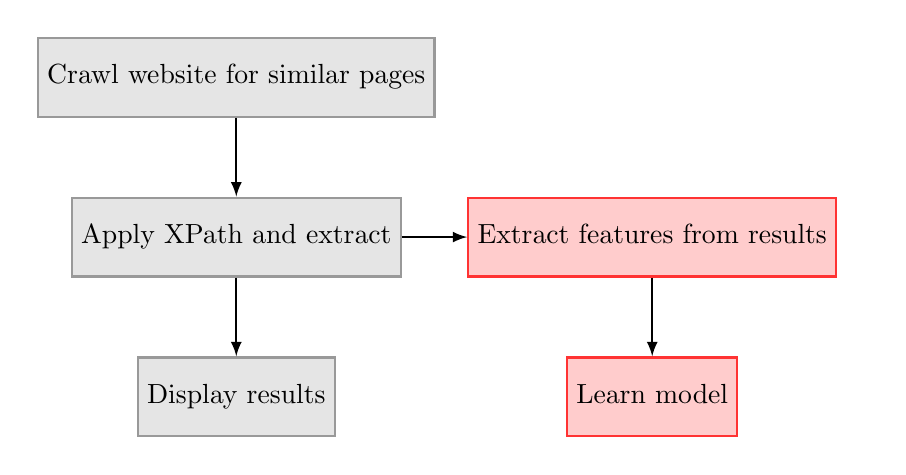
\begin{tikzpicture}[>=latex,text height=1.3ex,text depth=0.23ex]
  	\matrix[row sep=1cm,column sep=0.4cm]{
		\node (action1) [action]{Crawl website for similar pages}; 
		\\
		\node (action2) [action]{Apply XPath and extract}; &
		\node (ml1) [ml]{Extract features from results}; & 
		\\
		\node (action3) [action]{Display results}; &
		\node (ml2) [ml]{Learn model}; & 
		\\
	};
	\path[->]
	(action1) edge[thick] (action2)
	(action2) edge[thick] (action3)
	(action2) edge[thick] (ml1)
	(ml1)	edge[thick] (ml2)
	;
\end{tikzpicture}
\caption{Workflow of the machine learning component}
\label{fig:mlworkflow}
\end{figure}